%%%%%%%%%% Page 1 - Col 1 %%%%%%%%%%
\newpage
\colorfulheader{computer science}

\begin{minipage}[t]{0.485\textwidth}
    \colorfulsection{Bit Manipulation}
    \begin{customcenter}[2pt]
        \begin{tabular}{|c|c|c|c|c|c|}
             \hline
             \texttt{x} & \texttt{y} & \texttt{x \& y} & \texttt{x | y}& \texttt{x \string^ y} & {\raisebox{1.5pt}{\texttildelow}}\texttt{x} \\
             \hline
             1 & 1 & 1 & 1 & 0 & 0 \\
             \hline
             1 & 0 & 0 & 1 & 1 & 0 \\
             \hline
             0 & 1 & 0 & 1 & 1 & 1 \\
             \hline
             0 & 0 & 0 & 0 & 0 & 1 \\
             \hline
        \end{tabular}
    \end{customcenter}
    \colorfulsection{Data Structures}
    \begin{itemize}[leftmargin=*]
        \setlength\itemsep{0pt}
        \item A \textbf{linked list} can be implemented as
        \begin{customcenter}[-2pt]
            \begin{tabular}{|c|c|c|}
                \hline
                singly & doubly & circular \\
                \inlinecode{1->2->3->$\varnothing$} & \inlinecode{$\varnothing$<-1<->2<->3->$\varnothing$} & $\substack{\text{\inlinecode{1->2->3->1}} \\ \text{\inlinecode{1<->2<->3<->1}}}$ \\
                \hline
            \end{tabular}
        \end{customcenter}
        \item A \textbf{queue} can be done \textbf{circular}. The $n + 1$ element is inserted in the $0$ index if it is empty
        \item A \textbf{binary tree} (aka tree) is a hierarchical data structure where each node has \textbf{at most} 2 children
        \item Representation for binary tree
        \begin{customcenter}[-2pt]
            \begin{tabular}{|c|c|c|}
                \hline
                Data & Left child & Right child \\
                \inlinecode{node->data} & \inlinecode{node->left} & \inlinecode{node->right} \\
                \hline
            \end{tabular}
        \end{customcenter}
        \item Traversing a binary tree can be done as \\ 
        \textbf{Depth First}
        \begin{customcenter}[-2pt]
            \begin{tabular}{|c|c|c|}
                \hline
                Inorder & Preorder & Postorder \\
                (L-Root-R) & (Root-L-R) & (L-R-Root) \\
                \hline
            \end{tabular}
        \end{customcenter}
        \textbf{Breadth First} \\
        Level order
        \item Maximum number of nodes of tree at level $l$ is $2^l$
        \item For a tree of height $h$ $\mapsto$ maximum number of nodes is $2^{\parenthesisA{h + 1}} - 1$
        \item If not balanced the traversal complexity of a tree can be linear
        \item A \textbf{balanced binary tree} is a binary tree in which the height of the left and right subtrees at any node differ \textbf{at most by one}
        \item A \textbf{complete binary tree} has each level completely filled, except maybe for the last one which is partially filled left to right
        \begin{customcenter}[0pt]
            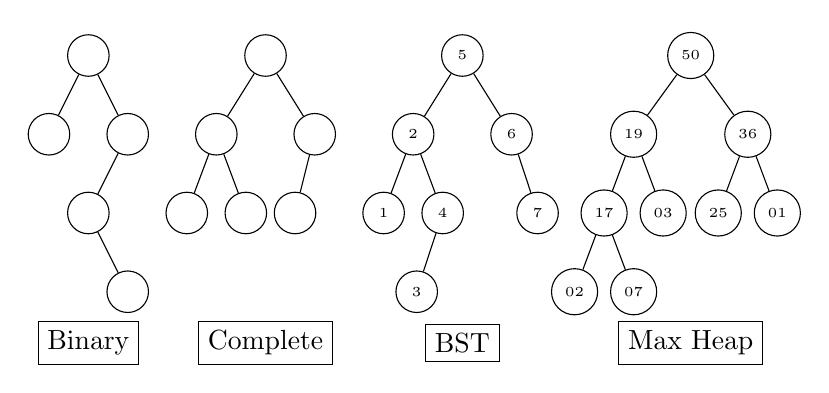
\begin{tikzpicture}
                \tikzstyle{treenode}=[circle,draw,minimum size=15pt]
                \draw[step=1cm,white,very thin] (0,0) grid (9.5,-4);
                \begin{scope}
                    \node[treenode] at (0.5, -0.35) {} [sibling distance=1.5cm]
                        child {
                            node[treenode,yshift=0.5cm,xshift=+0.25cm] {}
                            }
                        child {
                            node[treenode,yshift=0.5cm,xshift=-0.25cm] {}
                                child {
                                    node[treenode,xshift=-0.5cm,yshift=0.5cm] {}
                                        child {
                                            node[treenode,xshift=+0.5cm,yshift=0.5cm] {}
                                        }
                                }
                            };
                    \node[rectangle,draw] at (0.5, -4) {Binary};
                \end{scope}
                \begin{scope}
                    \node[treenode] at (2.75, -0.35) {} [sibling distance=1.75cm]
                        child {
                            node[treenode,yshift=0.5cm,xshift=+0.25cm] {}
                                child {
                                    node[treenode,yshift=0.5cm,xshift=+0.5cm] {}
                                }
                                child {
                                    node[treenode,yshift=0.5cm,xshift=-0.5cm] {}
                                }
                            }
                        child {
                            node[treenode,yshift=0.5cm,xshift=-0.25cm] {}
                                child {
                                    node[treenode,yshift=0.5cm,xshift=-0.25cm] {}
                                }
                        };
                    \node[rectangle,draw] at (2.75, -4) {Complete};
                \end{scope}
                \begin{scope}
                    \node[treenode] at (5.25, -0.35) {\tiny 5} [sibling distance=1.75cm]
                        child {
                            node[treenode,yshift=0.5cm,xshift=+0.25cm] {\tiny 2}
                                child {
                                    node[treenode,yshift=0.5cm,xshift=+0.5cm] {\tiny 1}
                                }
                                child {
                                    node[treenode,yshift=0.5cm,xshift=-0.5cm] {\tiny 4}
                                        child {
                                            node[treenode,yshift=0.5cm,xshift=-0.33cm] {\tiny 3}
                                        }
                                }
                            }
                        child {
                            node[treenode,yshift=0.5cm,xshift=-0.25cm] {\tiny 6}
                                child {
                                    node[treenode,yshift=0.5cm,xshift=+0.33cm] {\tiny 7}
                                }
                        };
                    \node[rectangle,draw] at (5.25, -4) {BST};
                \end{scope}
                \begin{scope}
                    \node[treenode] at (8.15, -0.35) {\tiny 50} [sibling distance=1.75cm]
                        child {
                            node[treenode,yshift=0.5cm,xshift=+0.15cm] {\tiny 19}
                                child {
                                    node[treenode,yshift=0.5cm,xshift=+0.5cm] {\tiny 17}
                                        child {
                                            node[treenode,yshift=0.5cm,xshift=+0.5cm]{\tiny 02}
                                        }
                                        child {
                                            node[treenode,yshift=0.5cm,xshift=-0.5cm]{\tiny 07}
                                        }
                                }
                                child {
                                    node[treenode,yshift=0.5cm,xshift=-0.5cm] {\tiny 03}
                                }
                            }
                        child {
                            node[treenode,yshift=0.5cm,xshift=-0.15cm] {\tiny 36}
                                child {
                                    node[treenode,yshift=0.5cm,xshift=+0.5cm] {\tiny 25}
                                }
                                child {
                                    node[treenode,yshift=0.5cm,xshift=-0.5cm] {\tiny 01}
                                }
                        };
                    \node[rectangle,draw] at (8.15, -4) {Max Heap};
                \end{scope}
            \end{tikzpicture}
        \end{customcenter}
        \vspace{-5pt}
        \item A \textbf{heap} is a data structure with the following properties
        \vspace{-5pt}
        \begin{enumerate}[leftmargin=*]
            \setlength\itemsep{0pt}
            \item A complete binary tree
            \item The value of each node must be no greater than (or no less than) the value of its child nodes
        \end{enumerate}
        \vspace{-5pt}
        \item A \textbf{binary search tree} (BST) has the following properties
        \vspace{-5pt}
        \begin{enumerate}[leftmargin=*]
            \setlength\itemsep{0pt}
            \item For each left subtree $\text{node}_l^{\text{value}} < \text{node}^{\text{value}}$
            \item For each right subtree has $\text{node}_r^{\text{value}} > \text{node}^{\text{value}}$
            \item The left and right subtree are also a BST
        \end{enumerate}
        \vspace{-5pt}
        \item A \textbf{graph} consist of \\ 
        1. Finite set of vertices called \textbf{nodes} \\ 
        2. Finite set of ordered pairs $\parenthesisA{u_i, v_j}$ called \textbf{edges} \\ \bracket{Directed graphs have $\parenthesisA{u_i, v_j}\neq\parenthesisA{v_j, u_i}$} \\ 
        3. An edge may contain a \textbf{weight} (also named value or cost)
    \end{itemize}
\end{minipage}
%%%%%%%%%%%%%%%%%%%%%%%%%%%%%%%%%%%%
\hspace{10pt}
%%%%%%%%%% Page 1 - Col 2 %%%%%%%%%%
\begin{minipage}[t]{0.485\textwidth}
    \begin{itemize}[leftmargin=*]
        \setlength\itemsep{0pt}
        \item Graphs are represented by $V\mapsto\text{Number of vertices}$ and $E\mapsto\text{Number of edges}$
        \item Graphs can be implemented as an \textbf{adjacency matrix} or as an \textbf{adjacency list}, having the following properties
    \end{itemize}
    \begin{customcenter}[3pt]
        \begin{tabular}{|c|c|c|}
        \hline
            \textbf{Graph Implementation} & \textbf{Traversal} & \textbf{Space}  \\
        \hline
            Matrix & $O\parenthesisA{V^2}$ & $O\parenthesisA{V^2}$ \\
        \hline
            List & $O\parenthesisA{V + E}$ & $O\parenthesisA{V + E}$ \\
        \hline
        \end{tabular}
    \end{customcenter}
    For example, given the following graph
    \begin{customcenter}[2pt]
        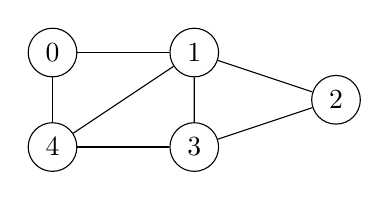
\begin{tikzpicture}[x=1cm, y=1cm, xscale=0.6, yscale=0.6, baseline=5.5pt]
        \node[circle, draw, minimum size=10pt] (c0) at (0,0){0}; 
        \node[circle, draw, minimum size=10pt] (c1) at (3,0){1}; 
        \node[circle, draw, minimum size=10pt] (c2) at (6,-1){2}; 
        \node[circle, draw, minimum size=10pt] (c3) at (3,-2){3}; 
        \node[circle, draw, minimum size=10pt] (c4) at (0,-2){4};
        \draw (c0) -- (c1);
        \draw (c0) -- (c4);
        \draw (c1) -- (c3);
        \draw (c4) -- (c1);
        \draw (c1) -- (c2);
        \draw (c2) -- (c3);
        \draw (c4) -- (c3);
        \end{tikzpicture}
    \end{customcenter}
    Can be represented as the matrix (right) or the list (left)\\
    \begin{minipage}[t]{0.485\textwidth}
        \vfill
        \centering
        \begin{tabular}{|c|ccccc|}
        \hline
        {} & 0 & 1 & 2 & 3 & 4 \\
        \hline
         0 & 0 & 1 & 0 & 0 & 1 \\
         1 & 1 & 0 & 1 & 1 & 1 \\
         2 & 0 & 1 & 0 & 1 & 0 \\
         3 & 0 & 1 & 1 & 0 & 1 \\
         4 & 1 & 1 & 0 & 1 & 0 \\
        \hline
        \end{tabular}
        \vfill
    \end{minipage}
    \begin{minipage}[t]{0.485\textwidth}
        \vfill
        \centering
        \begin{lstlisting}
            0 [] -> 1 [] -> 4 []
            1 [] -> 2 [] -> 3 [] -> 4 []
            2 [] -> 1 [] -> 3 []
            3 [] -> 1 [] -> 2 [] -> 4 []
            4 [] -> 3 [] -> 1 [] -> 0 []
        \end{lstlisting}
        \vfill
    \end{minipage}
    \emptyline
    \emptyline
    \colorfulsection{C Memory Layout}
    \begin{itemize}[leftmargin=*]
        \setlength\itemsep{0pt}
        \item Consists \quotes{typically} of 5 sections: 1. Text segment, 2. Initialized data segment, 3. Uninitialized data segment, 4. Heap, and 5. Stack
        \item The \textbf{text segment} contains the executable instructions. Can be places below the heap or stack regions. It is \textbf{read-only}
        \item \textbf{Initialized data segment} (or simply data segment) contains \textbf{global} and \textbf{static} variables \textbf{initialized by the programmer}. It can be subdivided in \textbf{read-only} and \textbf{read-write} areas. The following are examples of data segment \\ 
        \textcolor{white}{\hspace{1em}}\inlinecode{static int n = 10;}\\
        \textcolor{white}{\hspace{1em}}(defined anywhere)\\
        \textcolor{white}{\hspace{1em}}\inlinecode{const char * string = "hello world";}\\
        \textcolor{white}{\hspace{1em}}(defined outside the \inlinecode{main} function)
        \item \textbf{Uninitialized data segment} (or \quotes{block started by symbol} $\mapsto$ bss) contains \textbf{global} and \textbf{static} variables \textbf{not initialized explicitly} or initialized to zero. The following are examples of bss segment \\ 
        \textcolor{white}{\hspace{1em}}\inlinecode{static int i;}\\
        \textcolor{white}{\hspace{1em}}(defined anywhere)\\
        \textcolor{white}{\hspace{1em}}\inlinecode{int j;}\\
        \textcolor{white}{\hspace{1em}}(defined before the \inlinecode{main} function)
        \item The \textbf{stack} area contains the program stack (LIFO data structure) located in the higher parts of the memory (on x86 architecture it grows towards address zero). A set of values pushed for one function call is defined as \textbf{stack frame} (consisting at minimum of a return address). Each call to the stack allocates room for \textbf{automatic} and \textbf{temporary} variables. Allocation happens at \textbf{function call}
        \item The \textbf{heap} segment is where dynamic memory allocation takes place. Begins at the end of the bss segment and grows to larger addresses. In \inlinecode{C} language the heap area can be managed by \inlinecode{malloc, realloc} and \inlinecode{free} functions. \quotes{Contiguous} heap region is not mandatory for the previous C functions resulting in the possibility of \textbf{memory fragmentation}. Allocation happens at \textbf{execution of instruction}
    \end{itemize}
\end{minipage}
%%%%%%%%%%%%%%%%%%%%%%%%%%%%%%%%%%%%